\documentclass[xcolor=svgnames, aspectratio=169]{beamer}
\usepackage{pgfpages}
\setbeameroption{
  hide notes
  % show notes
  % show notes on second screen=right  % requires pgfpages
  % show only notes
}

\definecolor{mygreen}{rgb}{.125,.5,.25}

\setbeamertemplate{note page}{
  \vspace{.5cm}\hspace{.8\textwidth}
  \vspace{-2.7cm}
  \fbox{\insertslideintonotes{.2}}
  \pagecolor{white}
  \LARGE
  \begin{tikzpicture}[remember picture,overlay]
    \node [color=mygreen, opacity=0.8, xshift=-.3cm, yshift=-1.9cm, rotate=90] (current page.north west) {\bfseries N O T E S};
  \end{tikzpicture}
  \footnotesize
  \insertnote
}

% --- THEME ---
\usetheme[progressbar=frametitle]{metropolis}

\useoutertheme{metropolis}
\useinnertheme{metropolis}
\usefonttheme{metropolis}
\usecolortheme{spruce}  % spruce, metropolis, dove, crane, beaver, seagull
\setbeamercolor{background canvas}{bg=white}
\usecolortheme[named=mygreen]{structure}
\usefonttheme[onlymath]{serif}

% --- HACKS ---
% Hide numbers on standout slides.
\setbeamertemplate{frame numbering}{
    \ifbool{metropolis@standout}{}{
        \insertframenumber
    }
}
\setbeamertemplate{frame numbering}[counter]  % none, counter, fraction

% Avoid font-warning with itemize bullets.
\renewcommand\textbullet{\ensuremath{\bullet}}

% --- PACKAGES ---
\usepackage[UKenglish]{babel}
\usepackage[utf8]{inputenc}
\usepackage{lmodern}
\usepackage[T1]{fontenc}

% \usepackage{appendixnumberbeamer}
\usepackage{upquote}
\usetikzlibrary{positioning}
% \usepackage{minted}
\usepackage{multicol}
\usepackage{xspace}
\usepackage{booktabs}
\usepackage{siunitx}

% --- SETTINGS ---
\graphicspath{{./figures/}}
\setlength{\fboxsep}{0pt}

% --- OWN COMMANDS ---
\newcommand{\bdra}{\ensuremath{\boldsymbol \Rightarrow }~}
\newcommand{\dra}{\ensuremath{\Rightarrow }~}
\newcommand{\mr}[1]{\mathrm{#1}}
\newcommand{\emg}[2]{\texttt{emg#1#2}\xspace}
\newcommand{\empymod}{\texttt{empymod}\xspace}
\newcommand{\simpeg}{\texttt{SimPEG}\xspace}
\newcommand{\discretize}{\texttt{discretize}\xspace}
\newcommand{\custem}{\texttt{custEM}\xspace}
\newcommand{\petgem}{\texttt{PETGEM}\xspace}
\newcommand{\ohmm}{\ensuremath{\Omega\,}\text{m}\xspace}
\newcommand{\rmk}[1]{{\color{red}\bfseries #1}}
\newcommand{\maybe}[1]{{\color{gray} #1}}
\newcommand{\todo}{{\color{red}\texttt{TODO:}}\xspace}

% --- TITLE-STUFF ---
\title{Open-Source Landscape for Three-Dimensional Controlled-Source Electromagnetic Modeling\vspace{-1em}}
% \subtitle{}
\author{\vspace{-1em}
  Dieter Werthmüller\\
  Raphael Rochlitz\\
  Octavio Castillo Reyes\\
  Lindsey Heagy\\[1em]
  
\includegraphics[height=.7cm]{Logo-TUD}
  
\includegraphics[height=.5cm]{Logo-LIAG}\\
  
\includegraphics[height=.6cm]{Logo-BSC}
  
\includegraphics[height=.4cm]{Logo-BUC}\\
}
\date{\scriptsize 14th December 2020\\
  \maybe{\tiny
  \emph{Paper Number} GP005-06;
  \emph{Session} Frontiers in Electromagnetic (EM) Geophysics I;
  10:00--11:00 PST
 }
}

\institute{%
  \begin{tikzpicture}[remember picture,overlay]
    \node[xshift=.5\paperwidth, yshift=.66cm] at (current page.south west) {
\includegraphics[width=\paperwidth]{Logo-AGU}};
  \end{tikzpicture}
  \begin{tikzpicture}[remember picture,overlay]
    \node[xshift=.67\paperwidth, yshift=4.1cm] at (current page.south west) {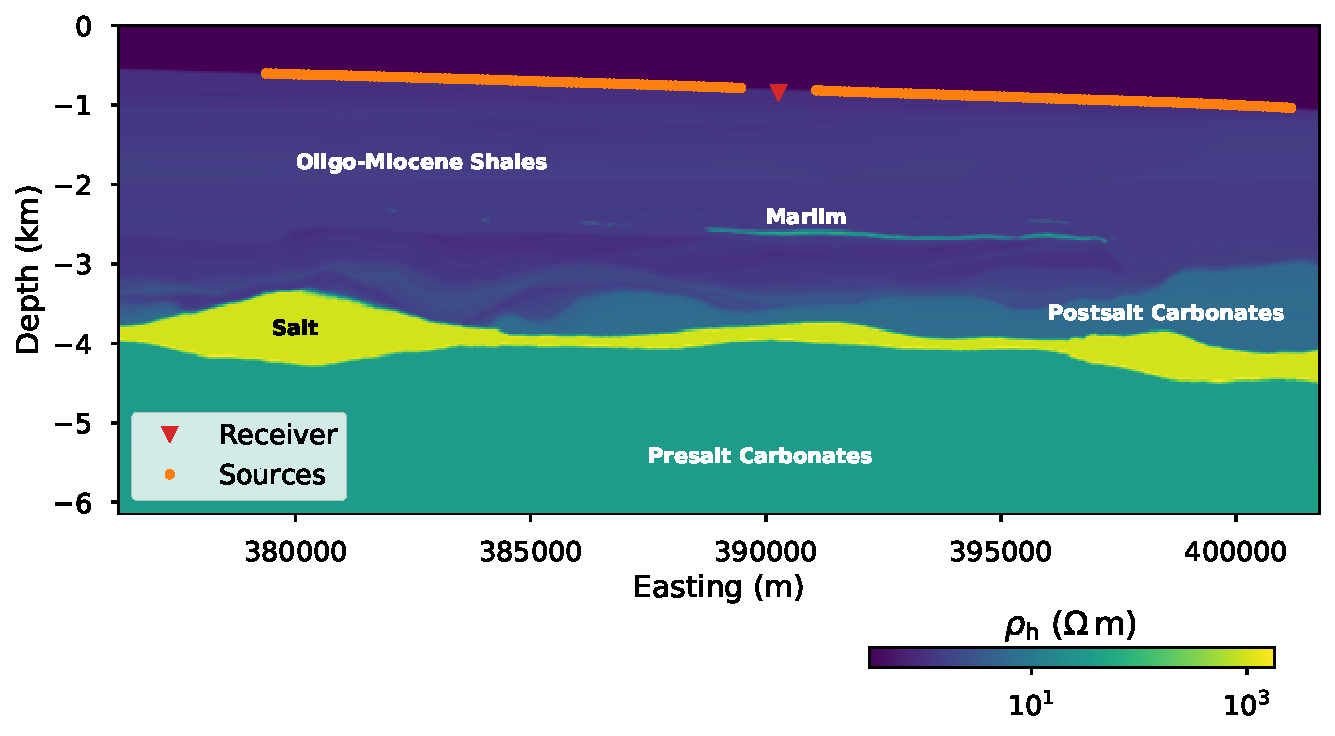
\includegraphics[width=.6\paperwidth]{model-marlim}};
  \end{tikzpicture}
}

% Title slide is one, so I want it to start at number 2 after the title.
\addtocounter{framenumber}{1}

% --- SLIDES ---
\begin{document}
\metroset{block=fill}  % Fills the block-environment

% guvcview for small video
% pdfpc for presenting
% - pdfpc 2020-12-14_Presentation.pdf --notes right -c  # Fails; then
% - pdfpc 2020-12-14_Presentation.pdf  -d 15
% vokoscreenNG for recording

% --------------------------------------------------------------------------- %
% - Presentation uploaded by Friday, 20/11                                    %
% - Max 15 minutes                                                            %
% - Maximum resolution: 1920x1080 pixels                                      %
% - Minimum resolution: 854x480 pixels                                        %
% - File format: MP4 (preferred), MOV, MPEG-2 or WebM                         %
% - Aspect ratio: 16:9 horizontal                                             %
% - reducing its size                                                         %
% - Maximum file size: 1 GB                                                   %
% --------------------------------------------------------------------------- %

% 01 -    01 : Title - Overview
% 02 -    02 : Intro to codes, problem
% 03 - 03-06 : Layered results
% 04 - 07-08 : Block results
% 05 -   -   : Marlim results
% 06 -       : Discussion
% 07 -       : Conclusions & Outlook
% 08 -       : References


\maketitle % ---------------------------------------------------------------- %
\note{
  \begin{itemize}
    \item Who am I, who are my co-authors
    \item What we have been working -- see MarlimR3D section:
      \begin{itemize}
        \item Open-source, huge resistivity model, 466 million cells
        \item 10, even 5 yrs ago impossible to simulate data\\
          with easily available open-source codes
        \item We look at four recent, open-source 3D CSEM codes; changes in the
          last years
        \item Able to model large-/industry-scale models
      \end{itemize}
    \item However, these new possibility open-up many more questions: How
      accurate are the results, what is the influence of the mesh type, etc.
    \item I will walk through the steps from
      \begin{itemize}
        \item verification (analytical solution),
        \item validation amongst codes (block), and
        \item validation with code from industry (MarlimR3D);
        \item discussion about mesh type;
        \item setting up simulation vs computation
      \end{itemize}
  \end{itemize}
}

\begin{frame}[c]%
  {Validation of large-scale 3D CSEM modelling using the\\
   open-source codes \custem, \emg3d, \petgem, and \simpeg}
  \vspace{.3cm}
  \begin{columns}[c]
    \column{.25\textwidth}
      \centering
      
\includegraphics[width=2.5cm]{Logo-emg3d}\\
      \href{https://empymod.github.io}{empymod.github.io}\\[.5cm]
      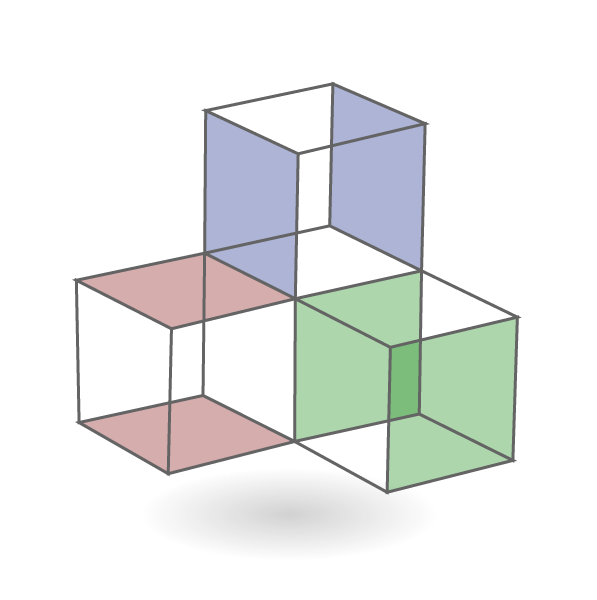
\includegraphics[width=2.5cm]{Logo-SimPEG}\\[-.4cm]
      \href{https://simpeg.xyz}{simpeg.xyz}\\[1cm]
    \column{.25\textwidth}
      \centering
      
\includegraphics[width=3.0cm]{Logo-PETGEM}\\
      \href{http://petgem.bsc.es}{petgem.bsc.es}\\[1cm]
      
\includegraphics[width=2.5cm]{Logo-custEM}\\
      \href{https://custem.rtfd.io}{custem.rtfd.io}\\[.5cm]~

    \column{.4\textwidth}
      \centering
      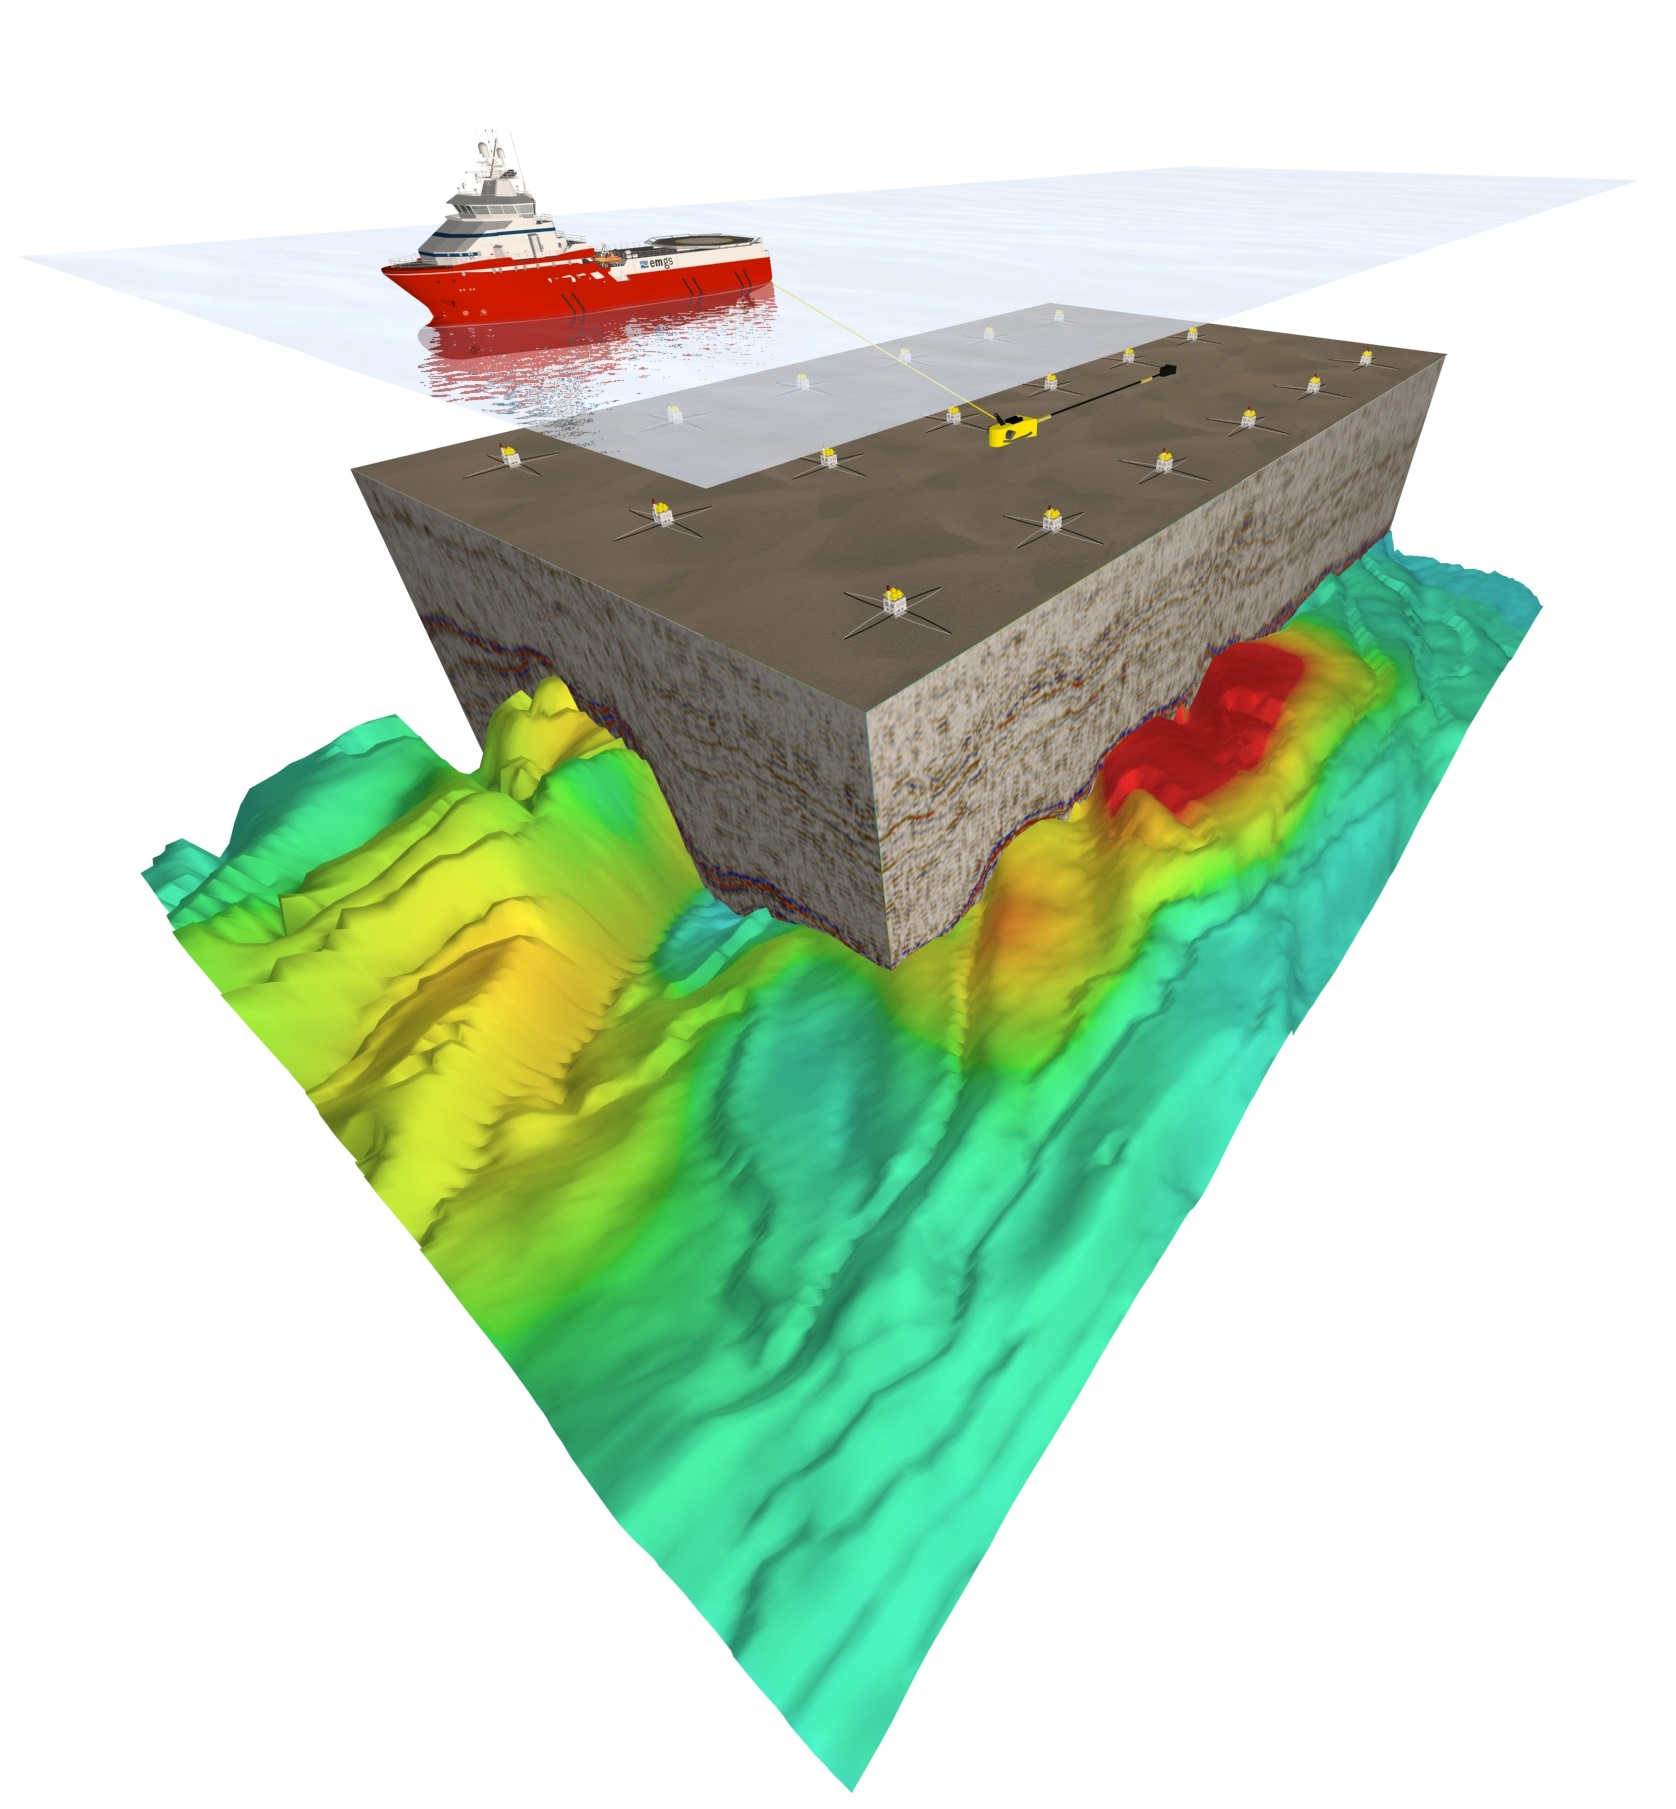
\includegraphics[width=\textwidth, trim=0 600 0 0, clip]{CSEM_Method3}
      \begin{tikzpicture}[remember picture,overlay]
        \node [color=white, xshift=1.5cm, yshift=1.4cm, rotate=60] (current page.south west) {\small \copyright\ emgs.com};
      \end{tikzpicture}
  \end{columns}
  \vspace{-.3cm}
  \small \alert{Werthmüller, Rochlitz, Castillo-Reyes, and Heagy, 2020},
  submitted to GJI; \href{https://arxiv.org/abs/2010.12926}{arXiv:~2010.12926}
  \note{
    \begin{itemize}
      \item We are core-devs of the four codes under consideration
      \item \custem and \petgem are finite element CSEM codes; both work in
        the\\ frequency domain, \custem also in the time domain; using
        tetrahedral meshes
      \item \simpeg is a more general framework for geophysical modelling and
        inversion:\\ Gravity, Magnetics, DC resistivity, IP, EM ($t$- and
        $f$-domain; controlled- and natural-src),\\ and more; contains
        1D, 2D, and 3D rectilinear, curvilinear, and octree meshes
      \item \emg3d is a matrix-free multigrid solver for 3D EM diffusion using
        rectilinear meshes.
      \item \custem, \petgem, and \simpeg use third party direct solvers such
        as MUMPS or PARDISO to solve the system of linear equations, \emg3d is
        a, iterative, solver on its own
      \item SimPEG is a community effort, other codes are currently mostly
        one-man shows
      \item Note: We look at the marine CSEM case as shown in the right figure;
        we are looking for resistive bodies in a conductive environment;
        node-based, using reciprocity; so just at one, tightly limited
        scenario; we will come back to that at the end
      \item Submitted to Geophysical Journal International, preprint on arXiv
      \item All are open-source: \simpeg MIT, \emg3d Apache-2.0, \petgem
        BSD-3-Clause, \custem GPL-3.0
    \end{itemize}
  }
\end{frame}

\section{Numerical Results} % ----------------------------------------------- %

\begin{frame}[t]%
  {Verification for layered model using semi-analytical solutions\\
   shows a relative amplitude error in the order of 1\,\% or less}
  %
  \begin{columns}[c]
    %
    \column{.45\textwidth}
    %
      \centering
      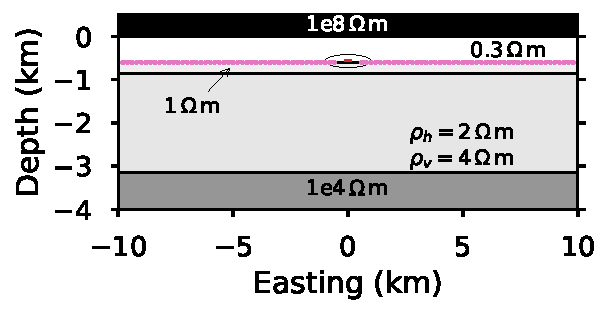
\includegraphics[width=\textwidth]{model-layered}\\
      \hspace{1cm}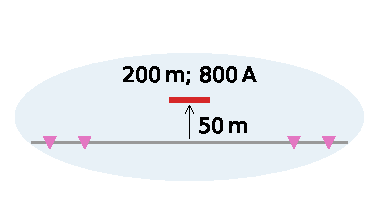
\includegraphics[width=.5\textwidth]{model-layered-src}
    %
    \column{.6\textwidth}
    %
      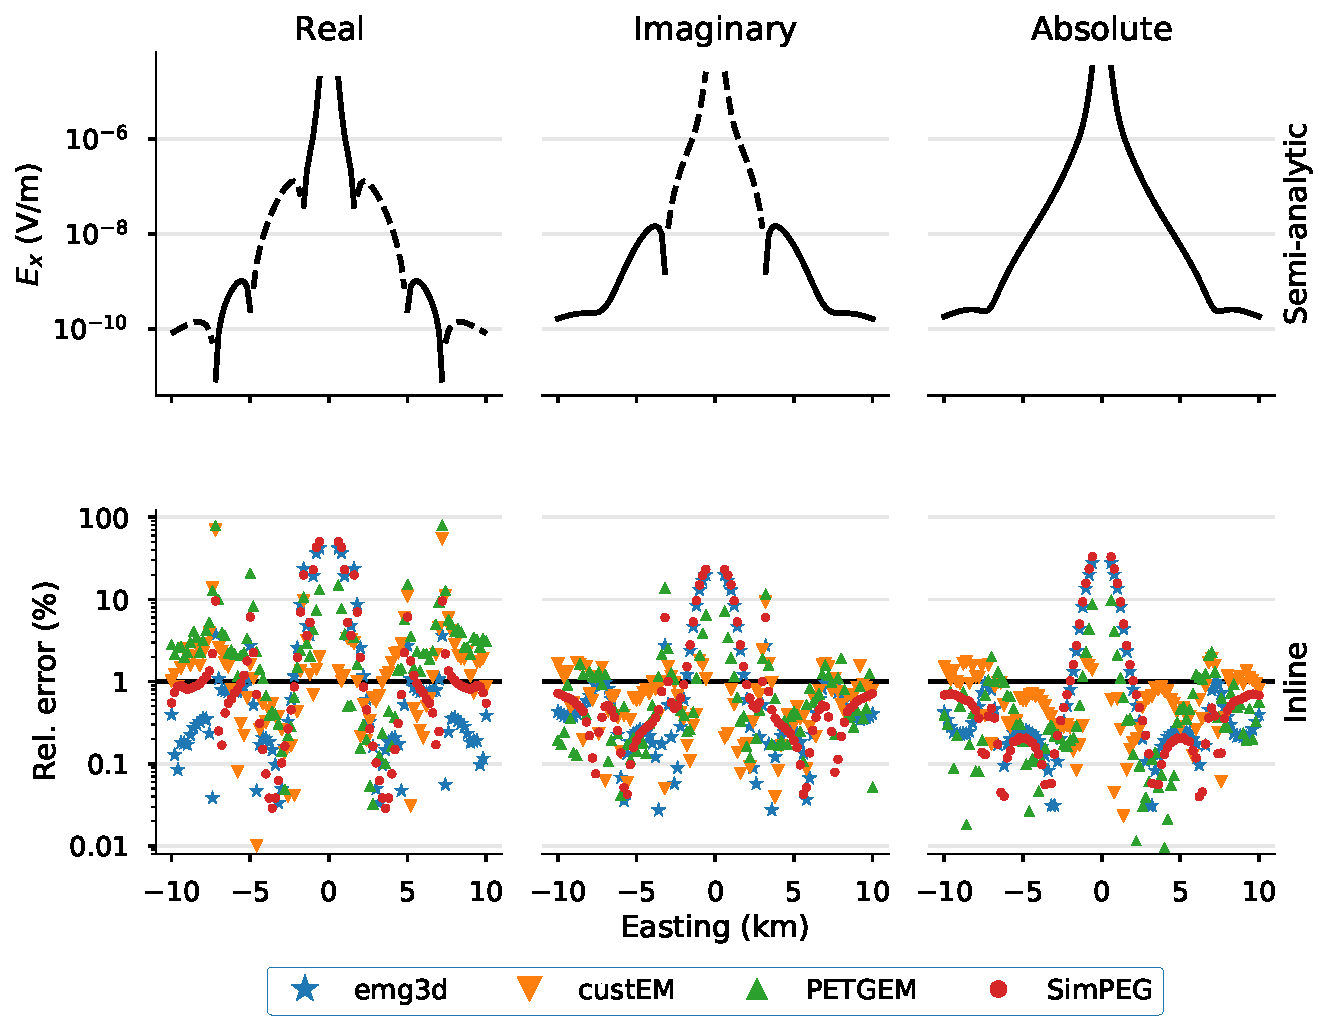
\includegraphics[width=\textwidth]{results-layered}
    %
  \end{columns}
  %
  \note{
    \begin{itemize}
      \item Source at x=8, 50\,m above seafloor; 200\,m, 800\,A, receivers on
        the seafloor
      \item Results of the four codes can visually not be distinguished
      \item Relative error from 0.01\,\% to 100\,\%
      \item Black lines mark the 1\,\% line
      \item The relative error of the amplitude is mostly below 1\,\%
      \item Looking at the absolute error plot now:
        \begin{itemize}
          \item Big relative errors can be observed close to the source
          \item Differences in how the source is defined
          \item Higher errors for \custem at the edges: explain the
            gridding approach of the thin layer of \custem
          \item Differences between PEC and PMC boundary conditions:
            \petgem and \emg3d used PEC, which seems to work better in this
            case, \simpeg and \custem used PMC
        \end{itemize}
      \item In paper also broadside; CPU/RAM/dof
      \item For the semi-analytical solutions we used \empymod
    \end{itemize}
  }
  %
\end{frame}

\begin{frame}[t]%
  {Adding three resistive blocks to the layered model requires\\
   the normalised difference instead of the relative error}
  %
  \begin{columns}[c]
    %
    \column{.6\textwidth}
      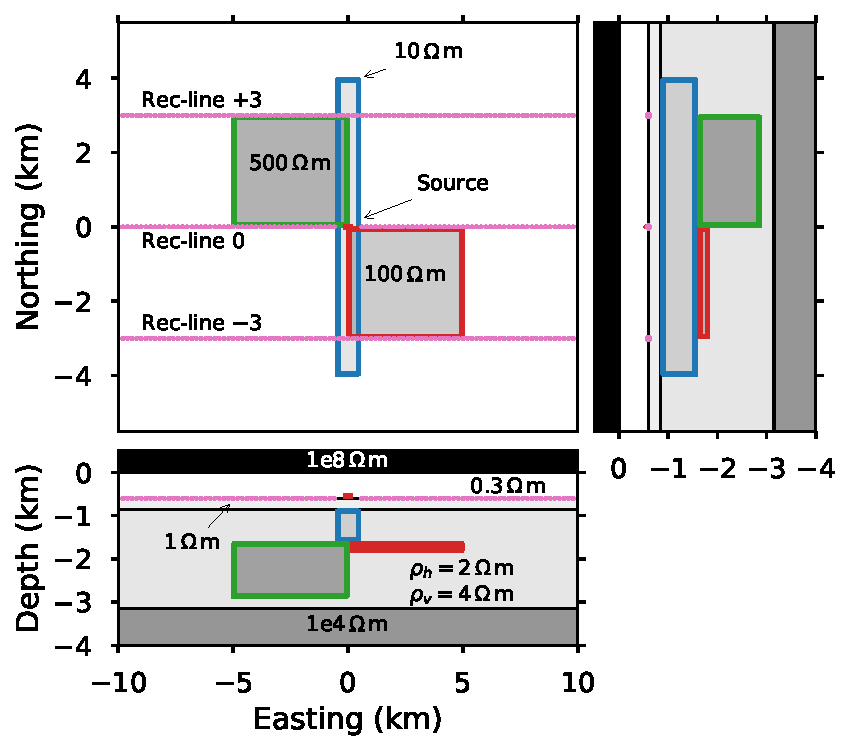
\includegraphics[width=.9\textwidth]{model-block}
    %
    \column{.4\textwidth}
      \centering
      \alert{Normalised Root-Mean Square Difference} (NRMSD) in
      percent:\\
      %
      \begin{equation}
        200\,\frac{|R_1 - R_2|}{|R_1| + |R_2|} \nonumber
      \end{equation}
      %
      \vspace{.5cm}\\
      %
      {\footnotesize After \emph{Dublin Test Model 1},\\
      \alert{Miensopust et al., 2013}, GJI}
    %
  \end{columns}
  %
  \note{
    \begin{itemize}
      \item Background model is the layered model from before
      \item We embed three resistive blocks and look at three acquisition
        lines
      \item The blocks are an adaption of the Dublin Test Model 1 from\\
        Miensopust et al., 2013; similar study for MT data
      \item As there are no analytical solutions we have to compare codes;\\
        hence \emph{validation}, not \emph{verification}
      \item Instead of the relative error we use therefore the NRMSD (and a
        conservative version thereof)
    \end{itemize}
  }
\end{frame}


% \begin{frame}[t]%
%   {Results from different meshes and different\\
%    codes can visually not be distinguished}
%   %
%   \vspace{.5cm}
%   \begin{columns}[c]
%     %
%     \column{.35\textwidth}
%       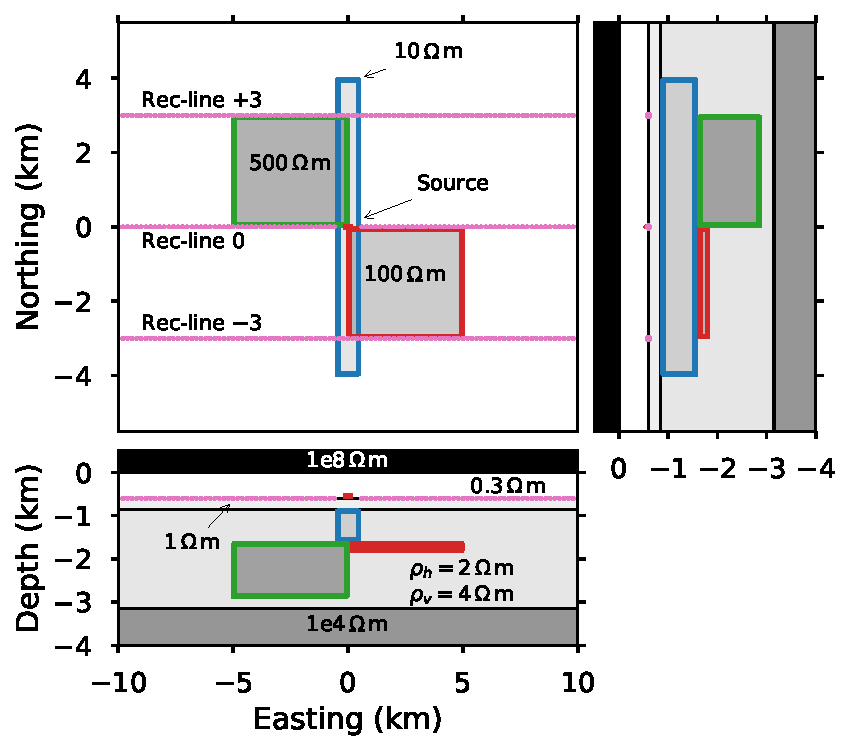
\includegraphics[width=.9\textwidth, trim=0 0 123.5 0, clip]{model-block}
%     %
%     \column{.65\textwidth}
%     %
%       \centering
%       \includegraphics[width=\textwidth]{results-block-all}\\
%       %
%       \vspace{ .5cm}
%       \begin{table}
%         \footnotesize %small %tiny
%         \begin{tabular}{lrS[table-format=6.0]S[table-format=4.1]S[table-format=8.0]}
%           % \begin{tabular}{lrrrr}
%           % \toprule
%           Code & \#Procs & {CPU (s)} & {RAM (GiB)}   & {\#dof} \\
%           \midrule
%           \custem & 24 &   158 & 115.9 & 1646736 \\
%           \emg3d  &  1 &   115 &   0.4 & 4813216 \\
%           \petgem & 24 &    238 &  152.8 & 2455868 \\
%           \simpeg &  4 & 10295 & 280.4 & 4813216 \\
%           % \bottomrule
%         \end{tabular}
%       \end{table}
%     %
%   \end{columns}
%   %
%   \note{
%     \begin{itemize}
%       \item Responses: Absolute values plotted
%       \item Plotted all results on top of each other: no differences visible
%       \item The responses of the resistive cubes are visible
%       \item Regarding computational costs:
%         \begin{itemize}
%           \item First: Comparison was not phrased as a comp. competition;
%             entire different exercise
%           \item Second: Ran on very different machines, from laptop to
%             supercomputers
%           \item The objective is: what can we do with different codes
%           \item How do we obtain good results with different codes
%           \item Much more time invested in model building than computation
%           \item \simpeg: fine grid (precision); later taking advantage of
%             octree meshes
%           \item Other three $\pm$ same speed in real-world
%             time, but \custem/\petgem used 24 processes
%           \item It can be directly seen for the direct solvers: more \#doc,
%             more RAM
%           \item Rectilinear grids required the most dofs
%           \item Layered model is basically identical
%         \end{itemize}
%     \end{itemize}
%   }
% \end{frame}


\begin{frame}[t]%
  {Validation between the codes shows a\\
   normalised difference of 1--2\,\% or less}
  %
  \vspace{.5cm}
  \begin{columns}[c]
    %
    \column{.35\textwidth}
      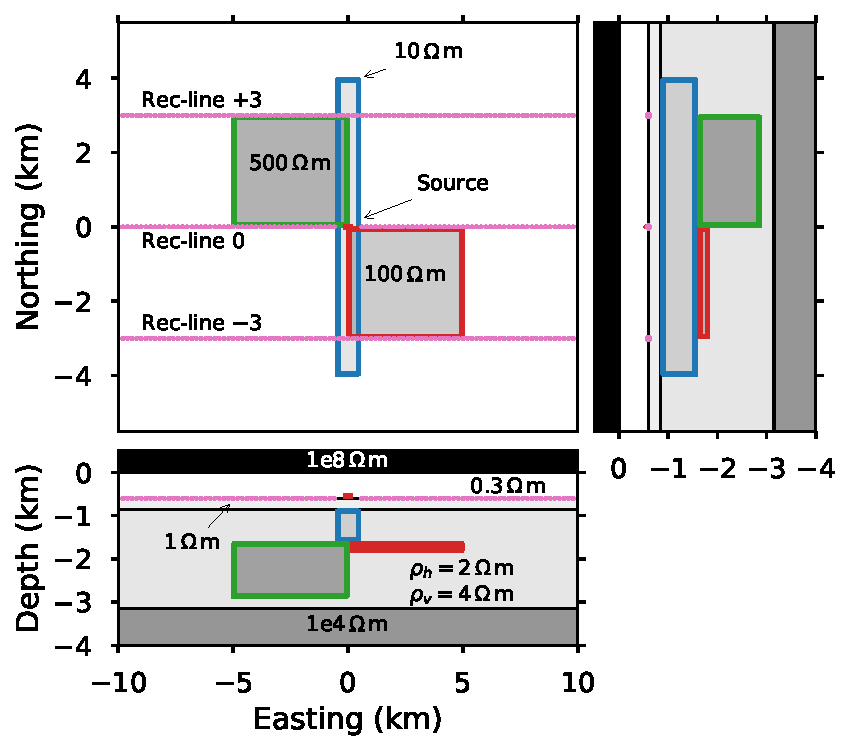
\includegraphics[width=.9\textwidth, trim=0 0 123.5 0, clip]{model-block}
    %
    \column{.65\textwidth}
    %
      % \includegraphics[width=\textwidth]{results-block-all-2}
      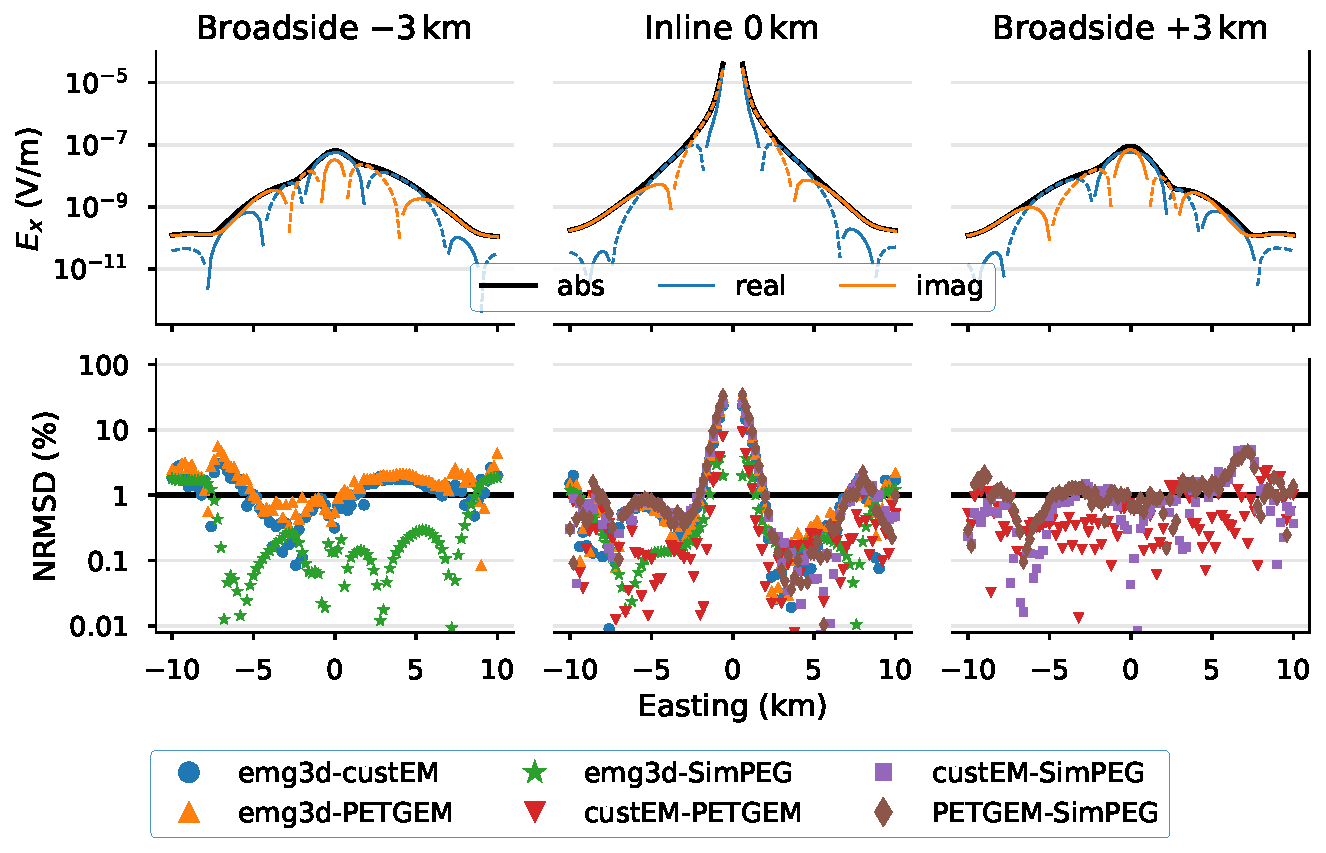
\includegraphics[width=\textwidth]{results-block}
    %
  \end{columns}
  %
  \note{
    \begin{itemize}
      \item Because they are basically identical, we just show the
        response of one code
      \item The responses of the resistive cubes are visible
      \item Shows also real and imaginary contributions
      \item The NRMSD is generally around 1\,\% or less
      \item Not surprising, as we could not see a visual difference
      \item There are 6 combinations for the normalized difference
        of the four codes
      \item Only middle plot shows all six
      \item On the left are three, on the right the other three
      \item \simpeg and \emg3d use same grid, so lower differences
      \item We use four different codes, two different mesh types, and the
        results are basically identical, which is a good first result
      \item Now we move to a huge model\ldots
    \end{itemize}
  }
\end{frame}


\begin{frame}[c]
  {Marlim R3D model: Responses at receiver locations\\
   look visually the same for all relevant responses}
  %
  \begin{columns}[c]
    \column{.5\textwidth}
      \centering
      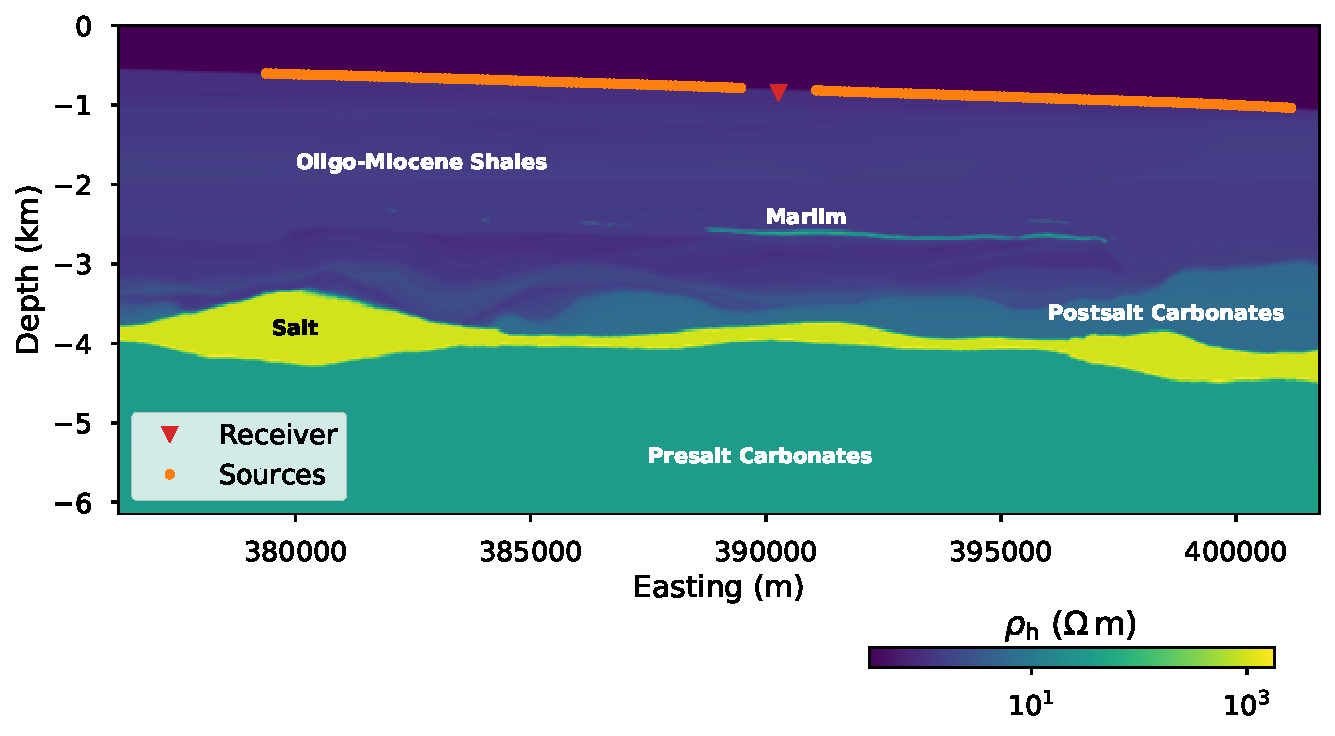
\includegraphics[width=\textwidth]{model-marlim}\\
      %
      {\footnotesize Marlim R3D:\\
        \alert{Correa and Menezes, 2019}, Geophysics}
    \column{.55\textwidth}
      \centering
      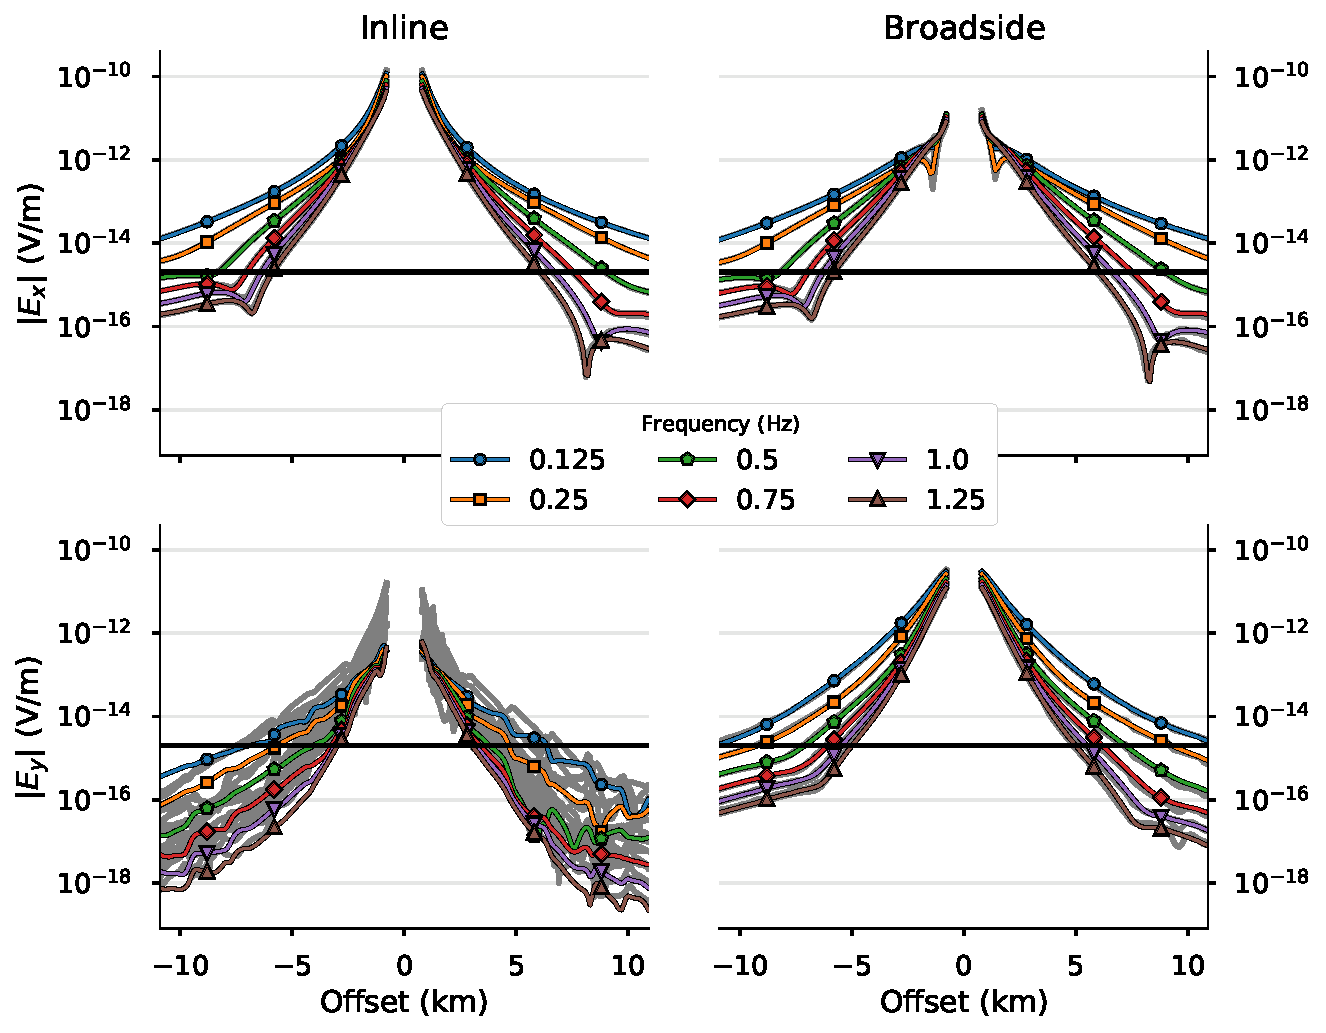
\includegraphics[width=\textwidth]{results-marlim-responses}
  \end{columns}
  \note{
    \begin{itemize}
      \item IMPORTANT: Reciprocity, hence source-receiver swap
      \item Very complex resistivity model
      \item Responses modelled with software from EMGS, in the time domain
      \item The responses look visually the same, except\ldots
      \item \ldots $E_x$ inline, which is about 2 orders of magnitudes lower
      \item Full grid of sources and receivers for 6 frequencies
      \item We modelled 1 receiver \dra source, two source \dra receiver lines
    \end{itemize}
  }
\end{frame}

\begin{frame}[c]
  {Normalised difference to published data is mostly\\
   below 10\,\% and very different from code to code}
  \centering
  %
  ~\vfill
  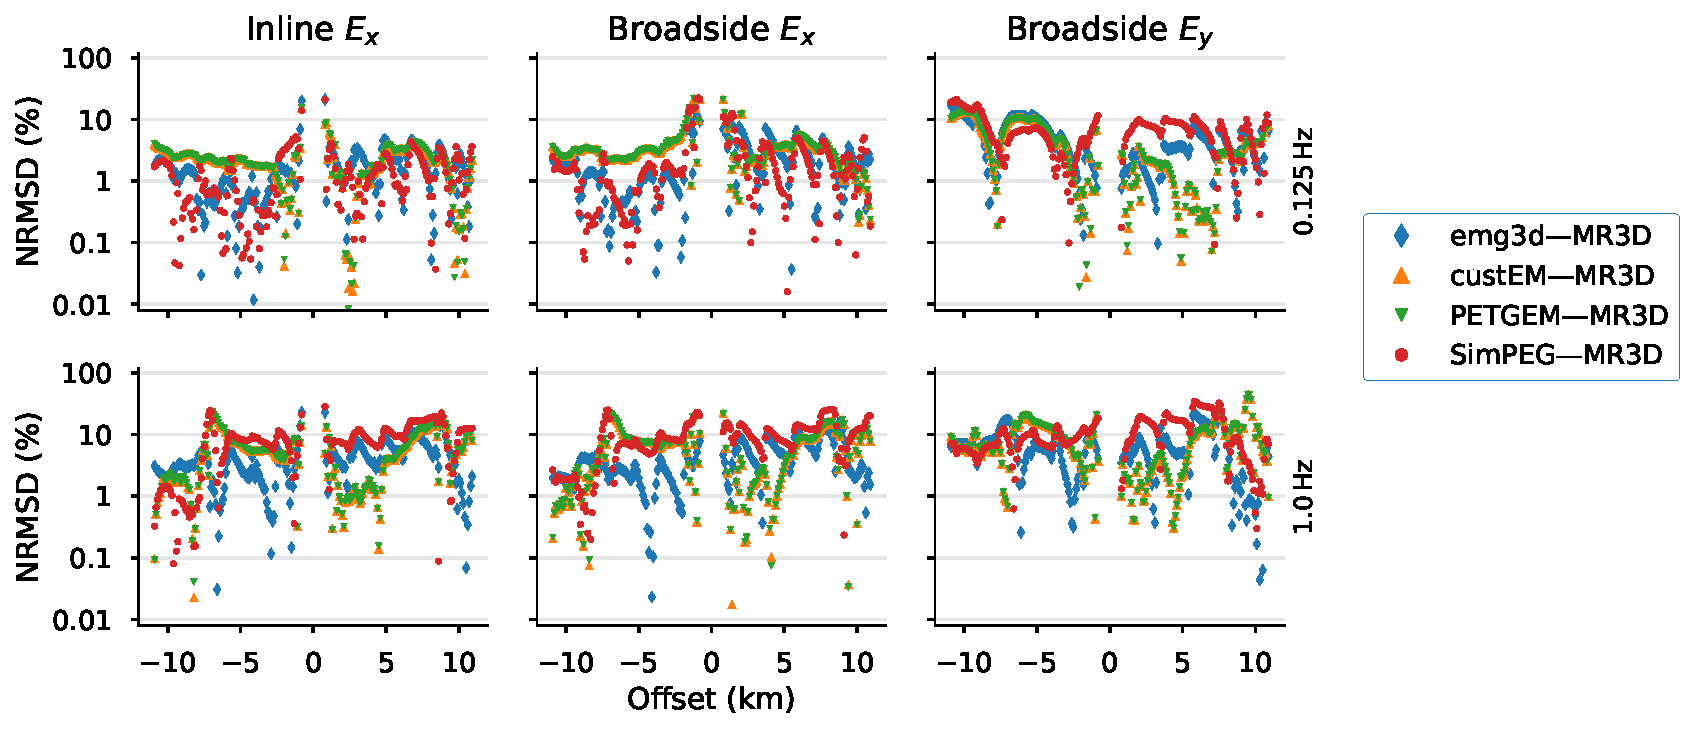
\includegraphics[width=\textwidth]{results-marlim_2published}
  %
  \note{
    \begin{itemize}
      \item $E_x$ inline, strongest component, a few percents
      \item Others up to 10 percent, higher frequencies more
      \item Some codes are more similar in different places
      \item funny shape due to bathymetry
    \end{itemize}
  }
\end{frame}

\begin{frame}[c]
  {Normalised difference between our codes\\
   is very similar and mostly below 10\,\%}
  \centering
  %
  ~\vfill
  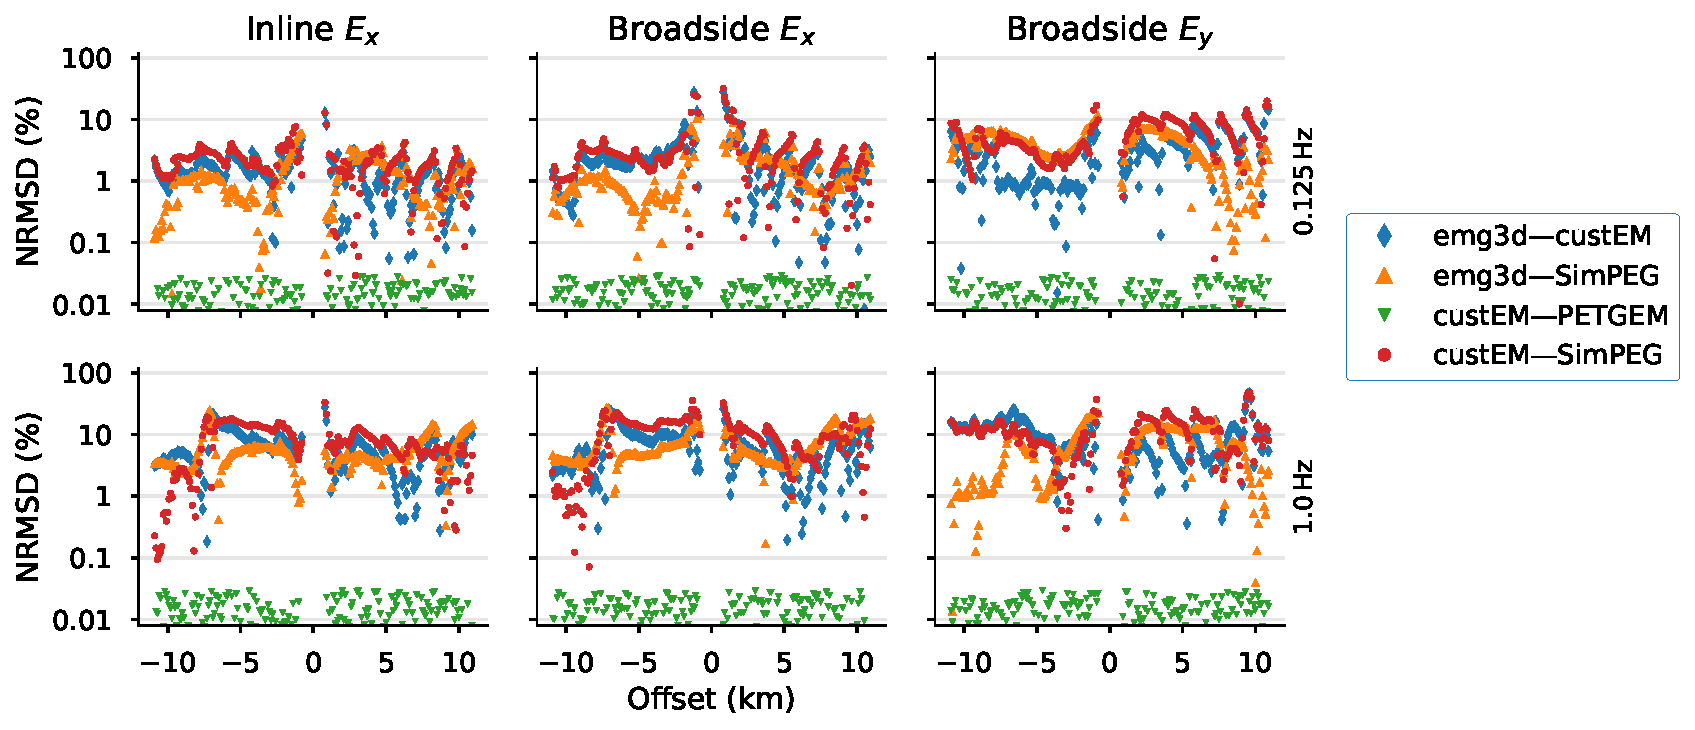
\includegraphics[width=\textwidth]{results-marlim_2ours}
  %
  \note{
    \begin{itemize}
      \item Comparison between our codes looks very similar
      \item Noteworthy is \custem and \petgem, because of same grid
      \item Also \emg3d and \simpeg, even though not same mesh
    \end{itemize}
  }
\end{frame}

% \begin{frame}
%   {Very insightful is to look at the entire\\
%    meshes and their different behaviours}
%   \centering
%   %
%   ~\vfill
%   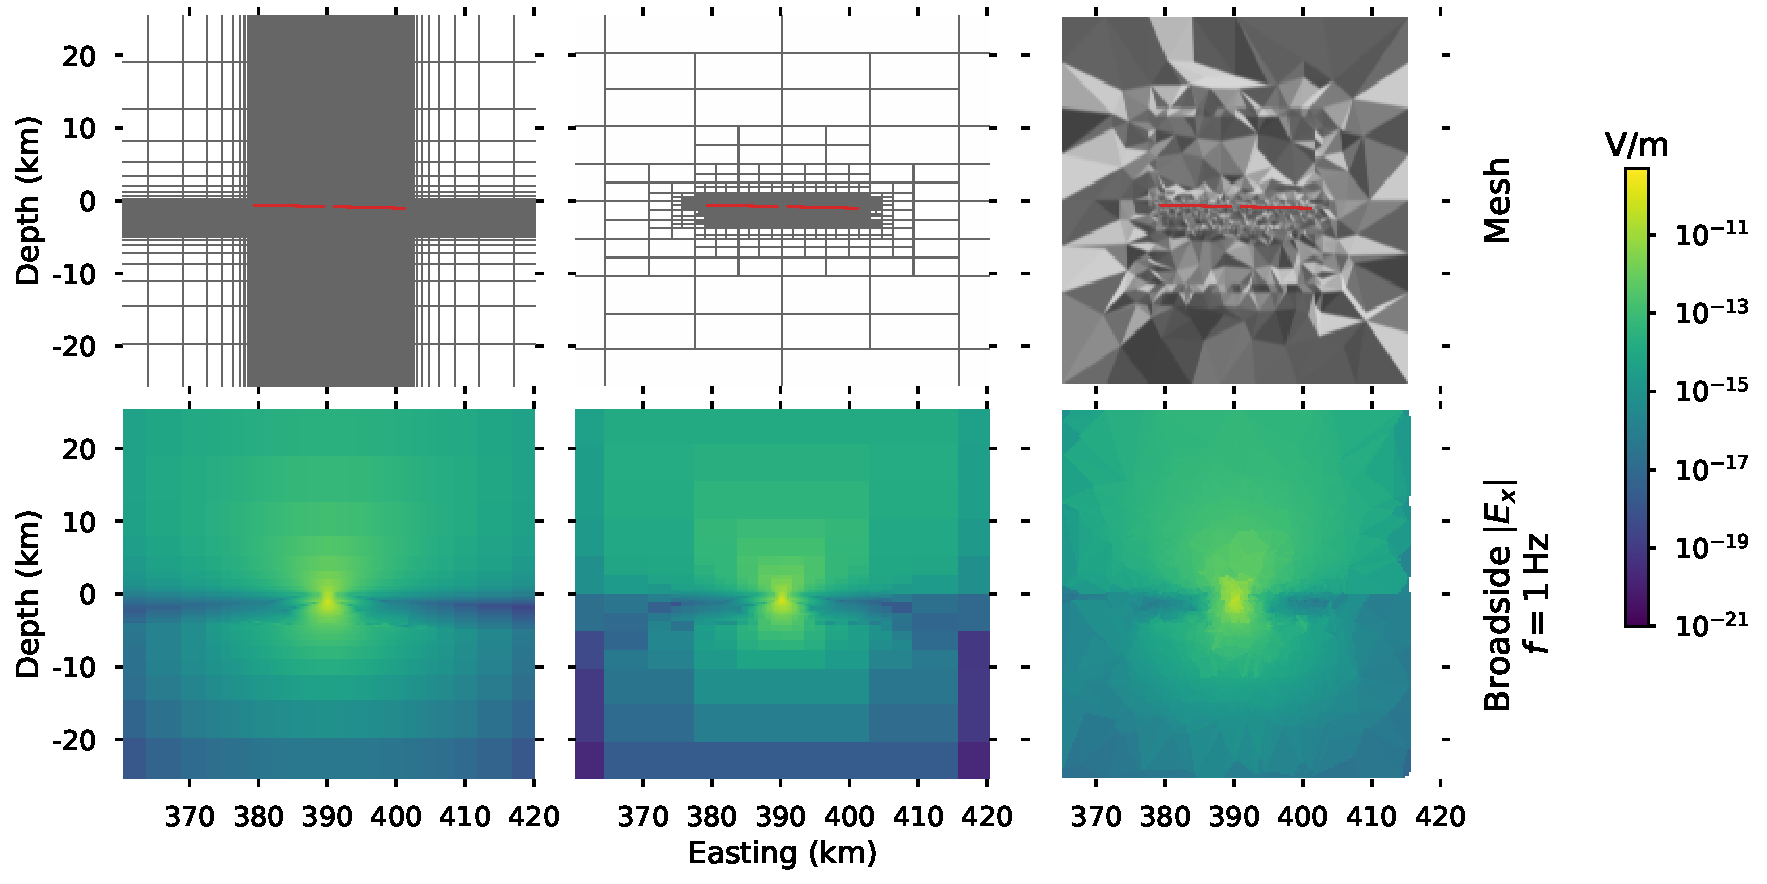
\includegraphics[width=.9\textwidth]{results-marlim_big}
%   %
%   \note{
%     \begin{itemize}
%       \item Computational domain very different
%       \item \simpeg and emg3d could probably reduce their domains
%       \item Advantages of Octree and Tetrahedra in comparison to Rectilinear
%     \end{itemize}
%   }
% \end{frame}

\begin{frame}
  {Very insightful is to look at the entire\\
   meshes and their different behaviours}
%   {While the responses at receiver locations are identical,\\
%    the fields start to vary greatly when moving away}
  \centering
  %
  ~\vfill
  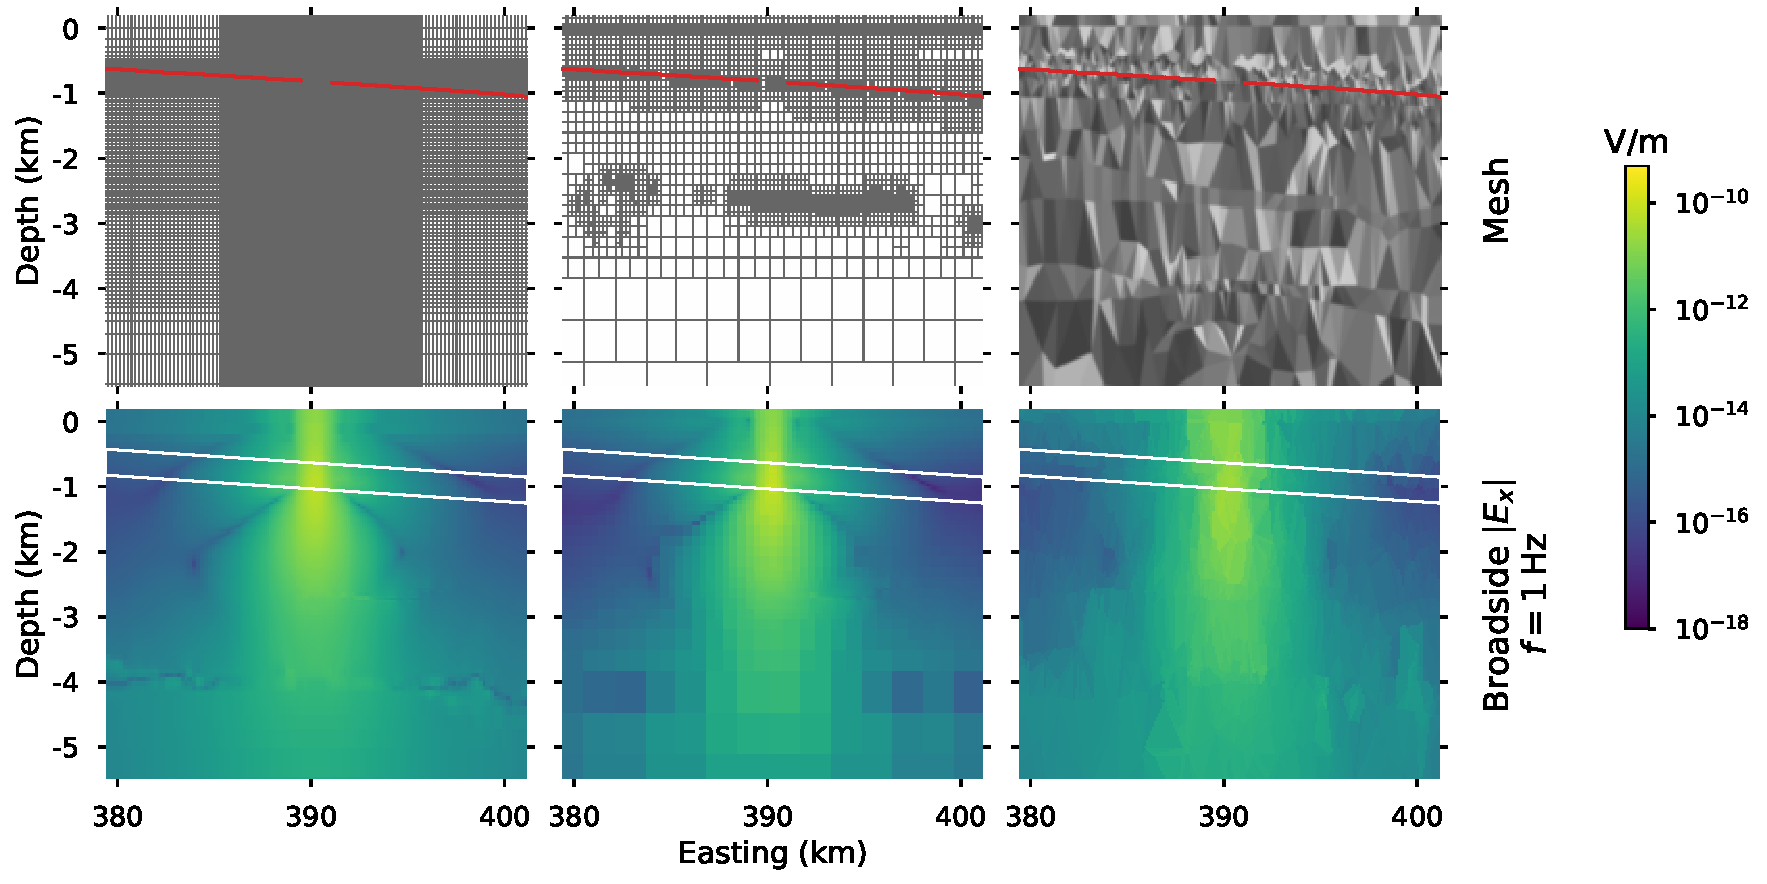
\includegraphics[width=.9\textwidth]{results-marlim_survey}
  %
  \note{
    \begin{itemize}
      \item White band includes the receiver lines
      \item Responses are very similar there
      \item Outside not so much!
      \item Very insightful for inversions etc
    \end{itemize}
  }
\end{frame}

\begin{frame}
  {A look at the models in different mesh yields interesting\\
   insights with regards to recoverability in inversions}
  \centering
  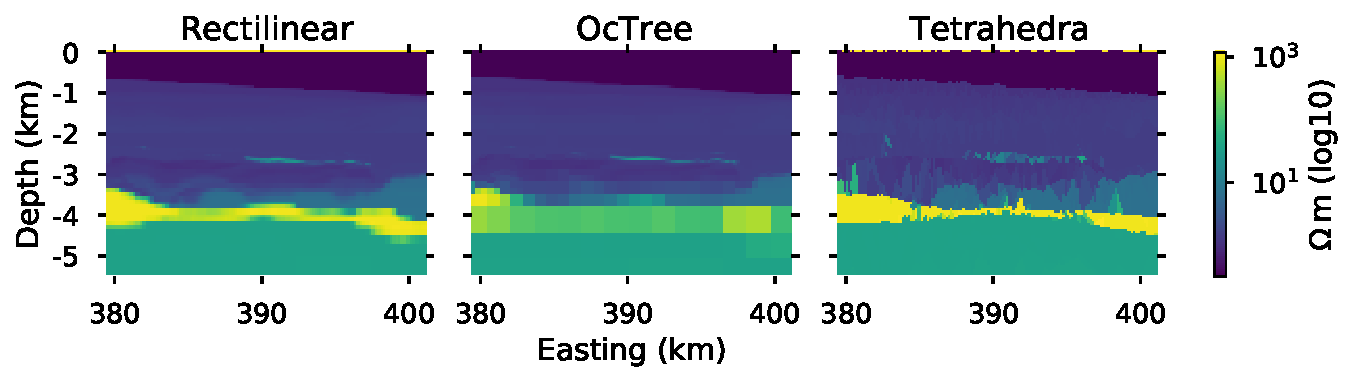
\includegraphics[width=\textwidth]{results-marlim_allmodels}
    \begin{table}
      \footnotesize %small %tiny
      \begin{tabular}{lrS[table-format=6.0]S[table-format=4.1]S[table-format=8.0]}
        % \begin{tabular}{lrrrr}
        % \toprule
        Code & \#Procs & {CPU (s)} & {RAM (GiB)}   & {\#dof} \\
        \midrule
        \custem & 64 &  872 & 230.1 & 1918106 \\
        \emg3d  &  1 & 1254 &   0.6 & 5998992 \\
        \petgem & 96 &  524 & 175.4 & 1918106 \\
        \simpeg &  4 &  422 &  12.8 &  720146 \\
        % \bottomrule
      \end{tabular}
    \end{table}
    \note{
      \begin{itemize}
        \item Models show clearly what we have seen before
        \item dof: tetrahedra about 2 million dofs, rectil. about 2 million
          cells; octree only about 240,000 cells
      \end{itemize}
    }
\end{frame}

\section{Conclusions and Outlook} % ----------------------------------------- %

\begin{frame}%
  {References}
  \tiny
  %
  \begin{columns}
    \column{1.1\textwidth}
  %
  \setlength{\columnseprule}{0.4pt}
  % \setlength{\columnsep}{3em}
  \begin{multicols}{2}
  A more extensive reference list can be found in:\\[.5em]
  {\bfseries \alert{Werthmüller, D., R. Rochlitz, O. Castillo-Reyes, and L.
  Heagy, 2020}, Open-source landscape for 3D CSEM modelling},\\
  submitted to Geophysical Journal International,
  \href{https://arxiv.org/abs/2010.12926}{arXiv:~2010.12926}.\\[.5cm]
  %
  {\bfseries Modelling codes: \custem, \emg3d, \petgem, \simpeg, and
  \empymod:}
  \begin{description}[2cm]
    %
    % \item[Castillo-Reyes et al., 2019,] {\bfseries Parallel 3D marine
    %   controlled-source electromagnetic modeling using high-order
    %   tetrahedral Nédélec elements}, Geophysical Journal International,
    %   219, 39--65,
    %   \href{https://doi.org/10.1093/gji/ggz285}{doi:~10.1093/gji/ggz285}.
    \item[Castillo-Reyes et al., 2018,] {\bfseries PETGEM: A parallel code
      for 3D CSEM forward modeling using edge finite elements}, Computers \&
      Geosciences, 119, 126--136,
      \href{https://doi.org/10.1016/j.cageo.2018.07.005}%
      {doi:~10.1016/j.cageo.2018.07.005}.
    %
    \item[Cockett et al., 2015,] {\bfseries SimPEG: An open source framework
      for simulation and gradient based parameter estimation in geophysical
      applications}, Computers \& Geosciences, 85, 142--154,
      \href{https://doi.org/10.1016/j.cageo.2015.09.015}%
      {doi:~10.1016/j.cageo.2015.09.015}.
    %
    \item[Rochlitz et al., 2019,] {\bfseries custEM: customizable finite
      element simulation of complex controlled-source electromagnetic data},
      Geophysics, 84, F17--F33,
      \href{https://doi.org/10.1190/geo2018-0208.1}%
      {doi:~10.1190/geo2018-0208.1}.
    %
    \item[Werthmüller, 2017,] {\bfseries An open-source full 3D
      electromagnetic modeler for 1D VTI media in Python: empymod},
      Geophysics, 82(6), WB9--WB19;
      \href{https://doi.org/10.1190/geo2016-0626.1}%
      {doi:~10.1190/geo2016-0626.1}.
    %
    \item[Werthmüller et al., 2019,] {\bfseries emg3d: A multigrid solver for
      3D electromagnetic diffusion}, Journal of Open Source Software, 4(39),
      1463;
      \href{https://doi.org/10.21105/joss.01463}{doi:~10.21105/joss.01463}.
    %
  \end{description}
  \columnbreak
  %
  {\bfseries Solvers \texttt{PETSc}, \texttt{MUPMS}, \texttt{FEniCS}, and
  \texttt{PARDISO}:}
  %
  \begin{description}[2cm]
    %
    \item[Abhyankar et al., 2018,] {\bfseries PETSc/TS: A modern scalable
      ODE/DAE solver library},
      \href{https://arxiv.org/abs/1806.01437}{arXiv:~1806.01437}.
    %
    \item[Amestoy et al., 2001,] {\bfseries A fully asynchronous multifrontal
      solver using distributed dynamic scheduling:} SIAM Journal on Matrix
      Analysis and Applications, 23, 15--41,
      \href{https://doi.org/10.1137/S0895479899358194}%
      {doi:~10.1137/S0895479899358194}.
    %
    \item[Langtangen et al., 2016,] {\bfseries Solving PDEs in Python: The
      FEniCS Tutorial I}, vol. 3 of Simula SpringerBriefs on Computing,
      Springer International Publishing,
      \href{https://doi.org/10.1007/978-3-319-52462-7}%
      {doi:~10.1007/978-3-319-52462-7}.
    %
    \item[Schenk and Gärtner, 2004,] {\bfseries Solving unsymmetric sparse
      systems of linear equations with PARDISO}, Future Generation Computer
      Systems, 20, 475--487,
      \href{https://doi.org/10.1016/j.future.2003.07.011}%
      {doi:~10.1016/j.future.2003.07.011}.
    %
  \end{description}
  %
  {\bfseries Marlim R3D model:}
  %
  \begin{description}[2cm]
    %
    \item[Correa and Menezes, 2019,] {\bfseries Marlim R3D: A realistic model
      for controlled-source electromagnetic simulations--Phase 2: The
      controlled-source electromagnetic data set}, Geophysics, 84,
      E293--E299, \href{https://doi.org/10.1190/geo2018-0452.1}%
      {doi:~10.1190/geo2018-0452.1}.
    %
  \end{description}
  %
  {\bfseries MT comparison study:}
  %
  \begin{description}[2cm]
    %
    \item[Miensopust et al., 2013,] {\bfseries Magnetotelluric 3-D inversion--a
      review of two successful workshops on forward and inversion code testing
      and comparison}, Geophysical Journal International, 193, 1216--1238,
      \href{https://doi.org/10.1093/gji/ggt066}{doi: 10.1093/gji/ggt066}.
    %
  \end{description}
  %
\end{multicols}
\end{columns}
\end{frame}

\begin{frame}[c]%  {}
  {More Comparisons \& Benchmarks\\
   Other Scenarios, other programming languages}
  %
  \begin{columns}
      %
    \column{.2\textwidth}
    \centering
      %
      ~\\[.5cm]
      
\includegraphics[width=2.0cm]{Logo-emg3d}\\[.5cm]
      %
      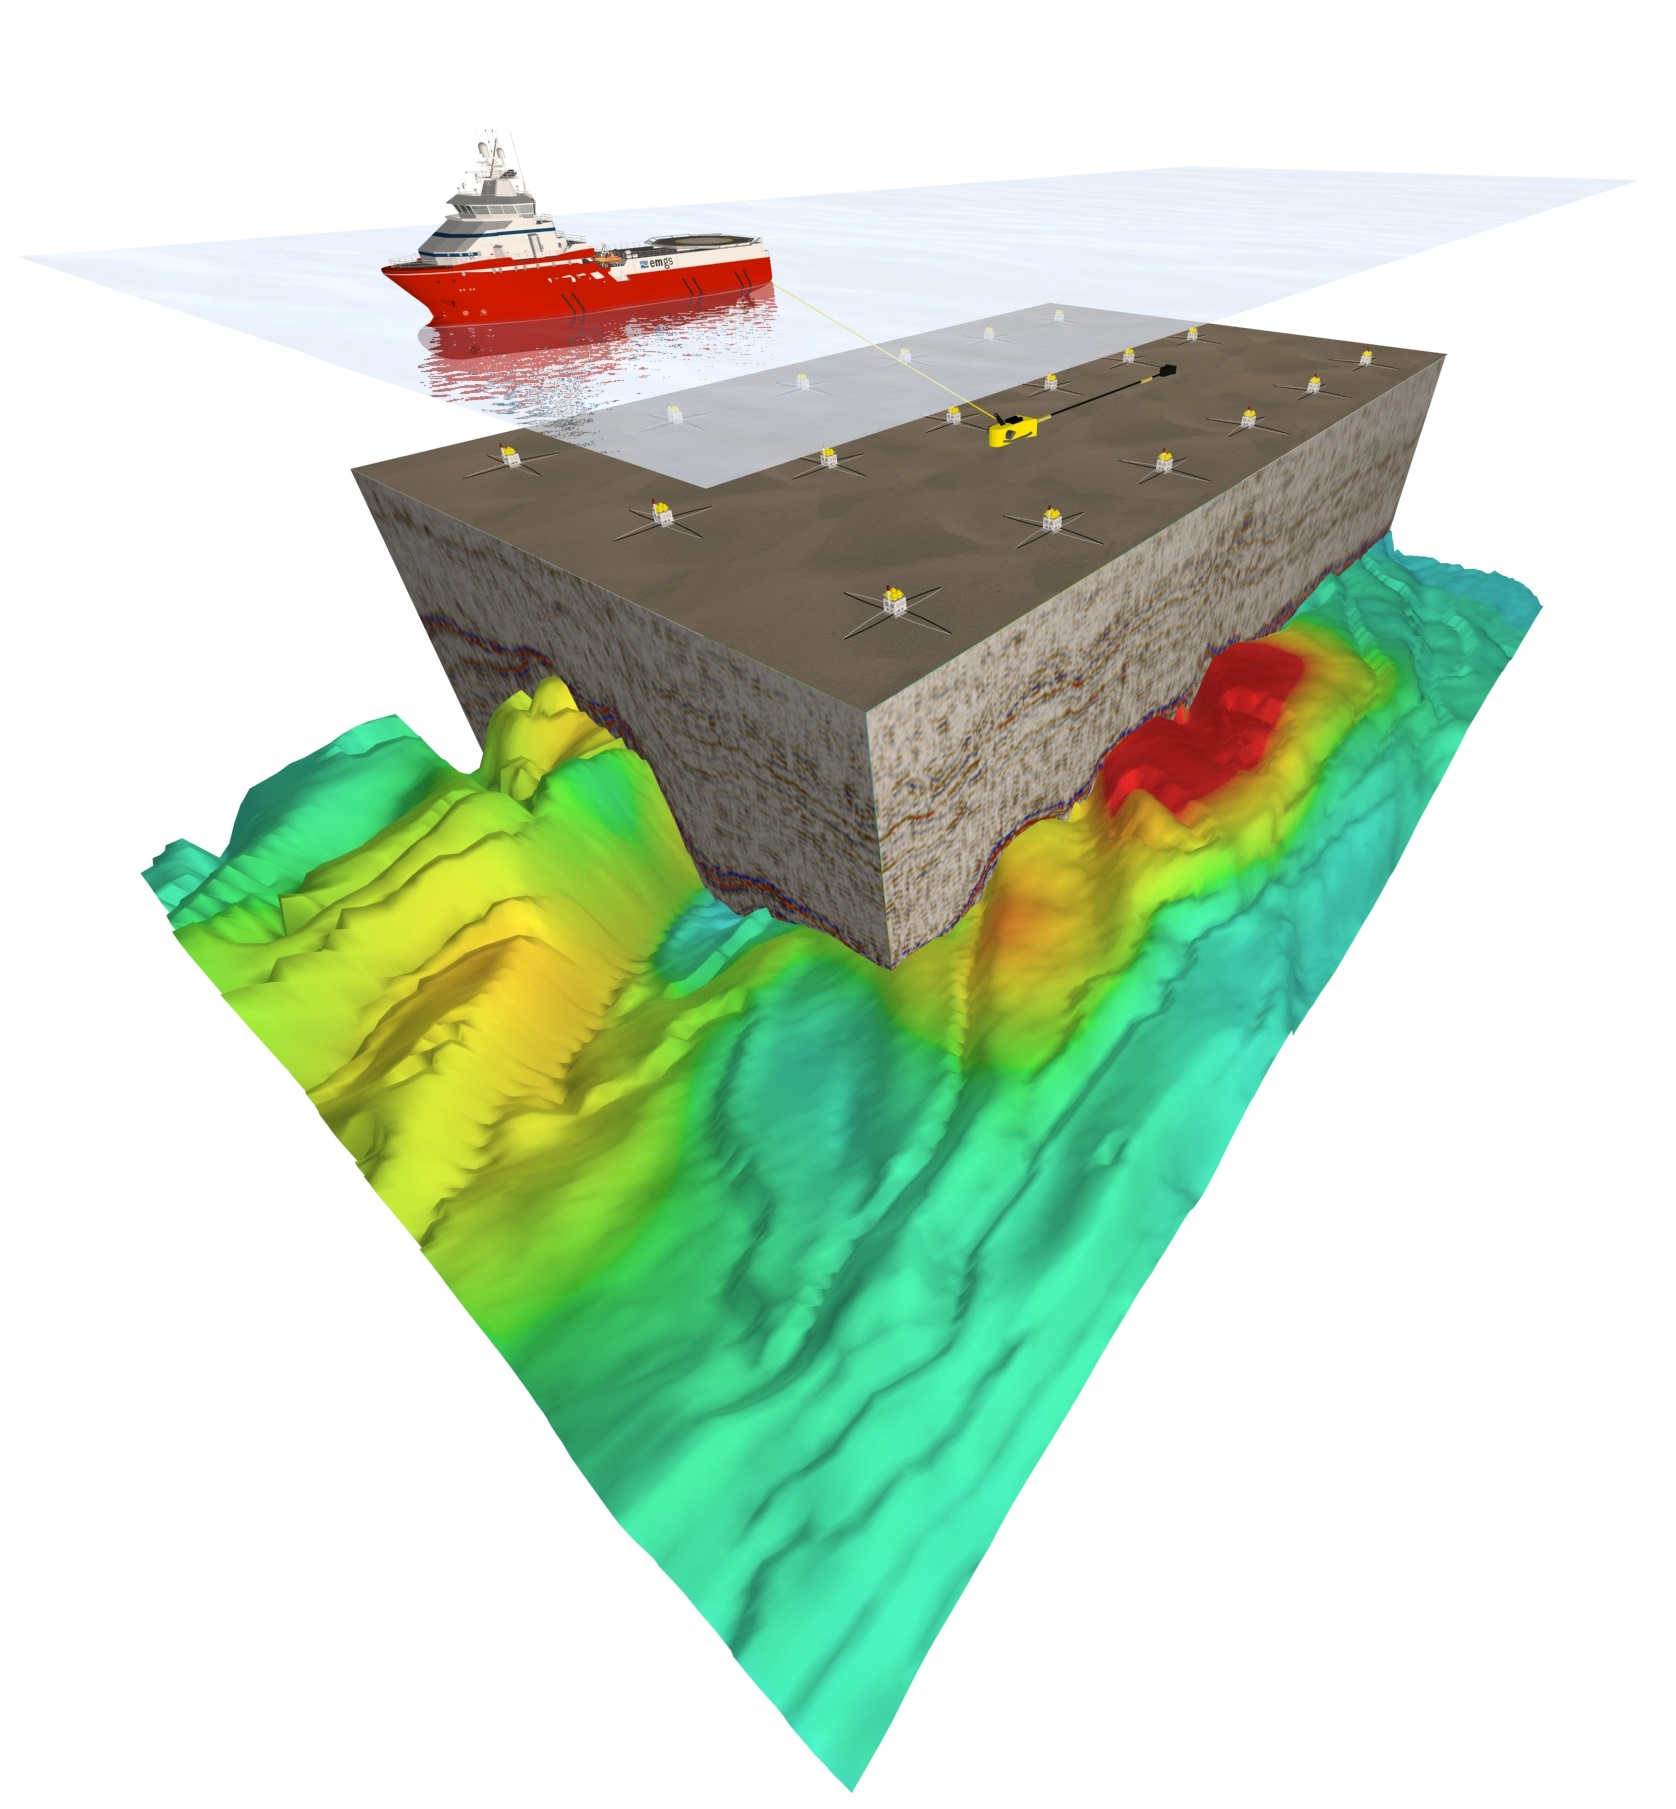
\includegraphics[width=\textwidth, trim=0 500 0 0, clip]{CSEM_Method3}\\[1cm]
      %
      
\includegraphics[width=2.0cm]{Logo-custEM}
      %
    \column{.5\textwidth}
    \centering
      %
    \phantom{~}\\[.5cm]
    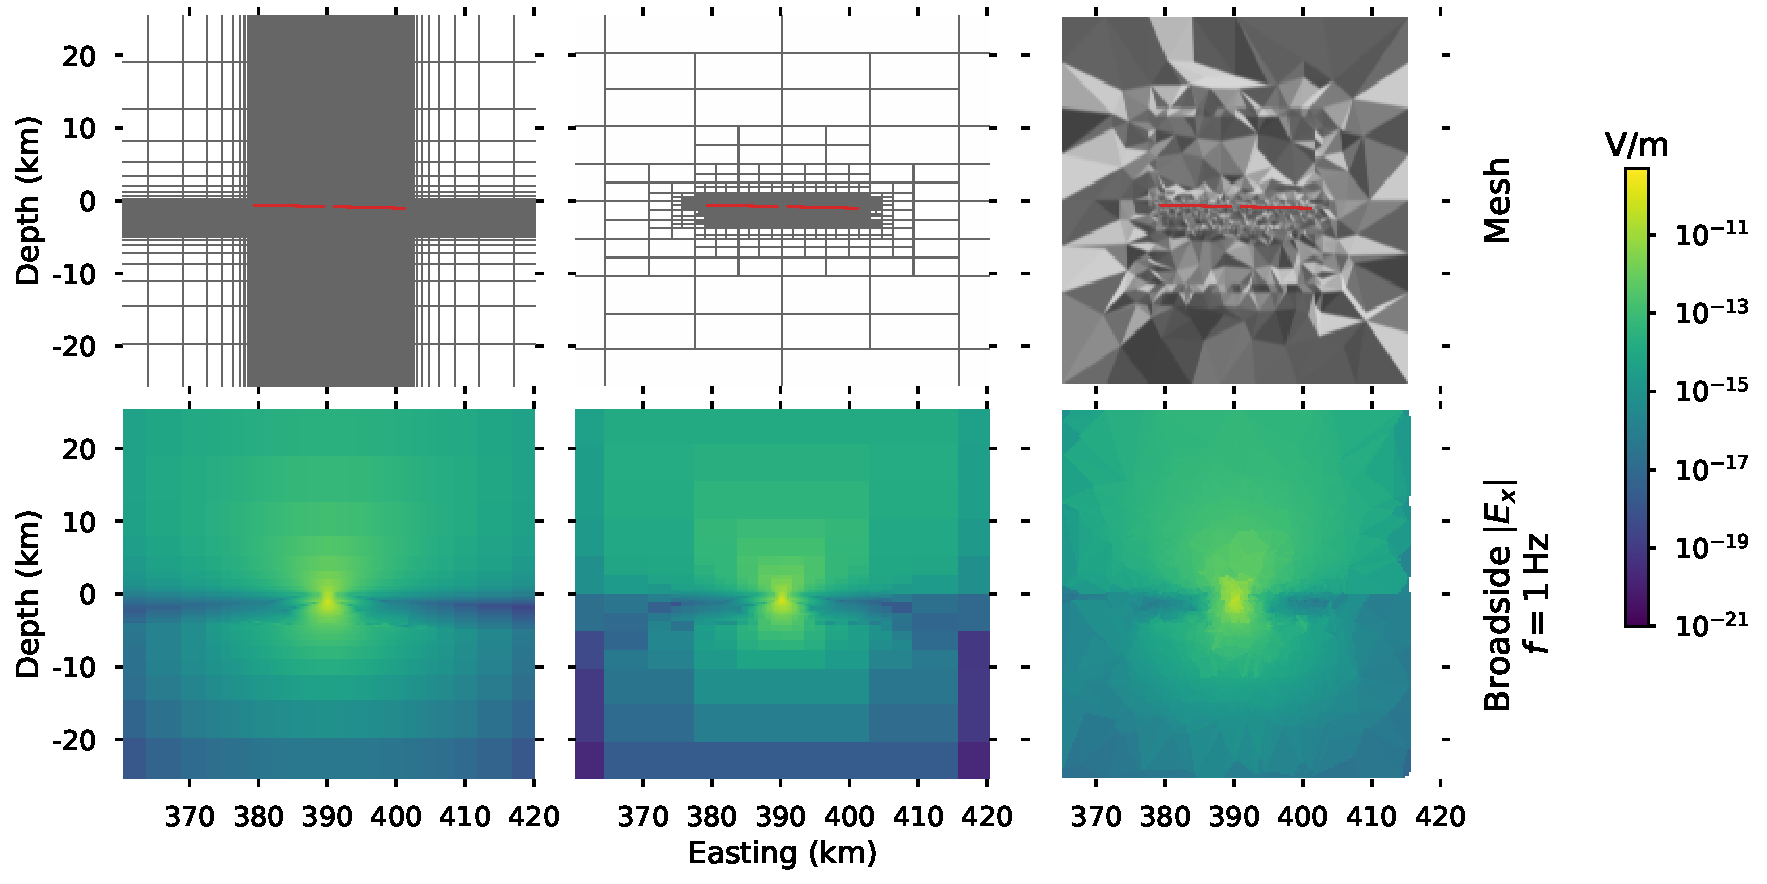
\includegraphics[width=\textwidth, trim=40 235 150 0, clip]{results-marlim_big}\\[.5cm]
      %
      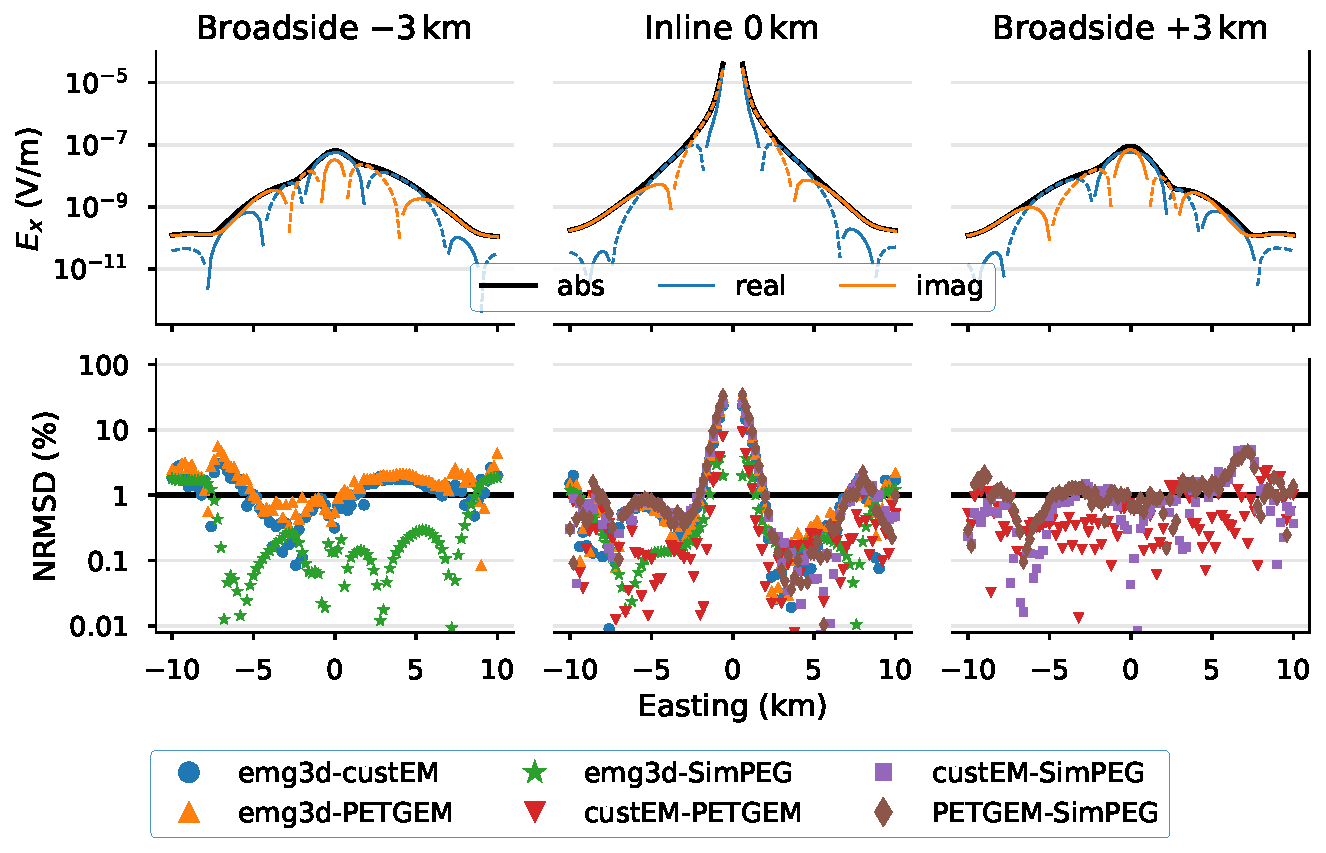
\includegraphics[width=\textwidth, trim=70 095 0 160, clip]{results-block}
      %
    \column{.3\textwidth}
    \centering
      %
      
\includegraphics[width=3cm]{Logo-SimPEG2}\\[.5cm]
      %
      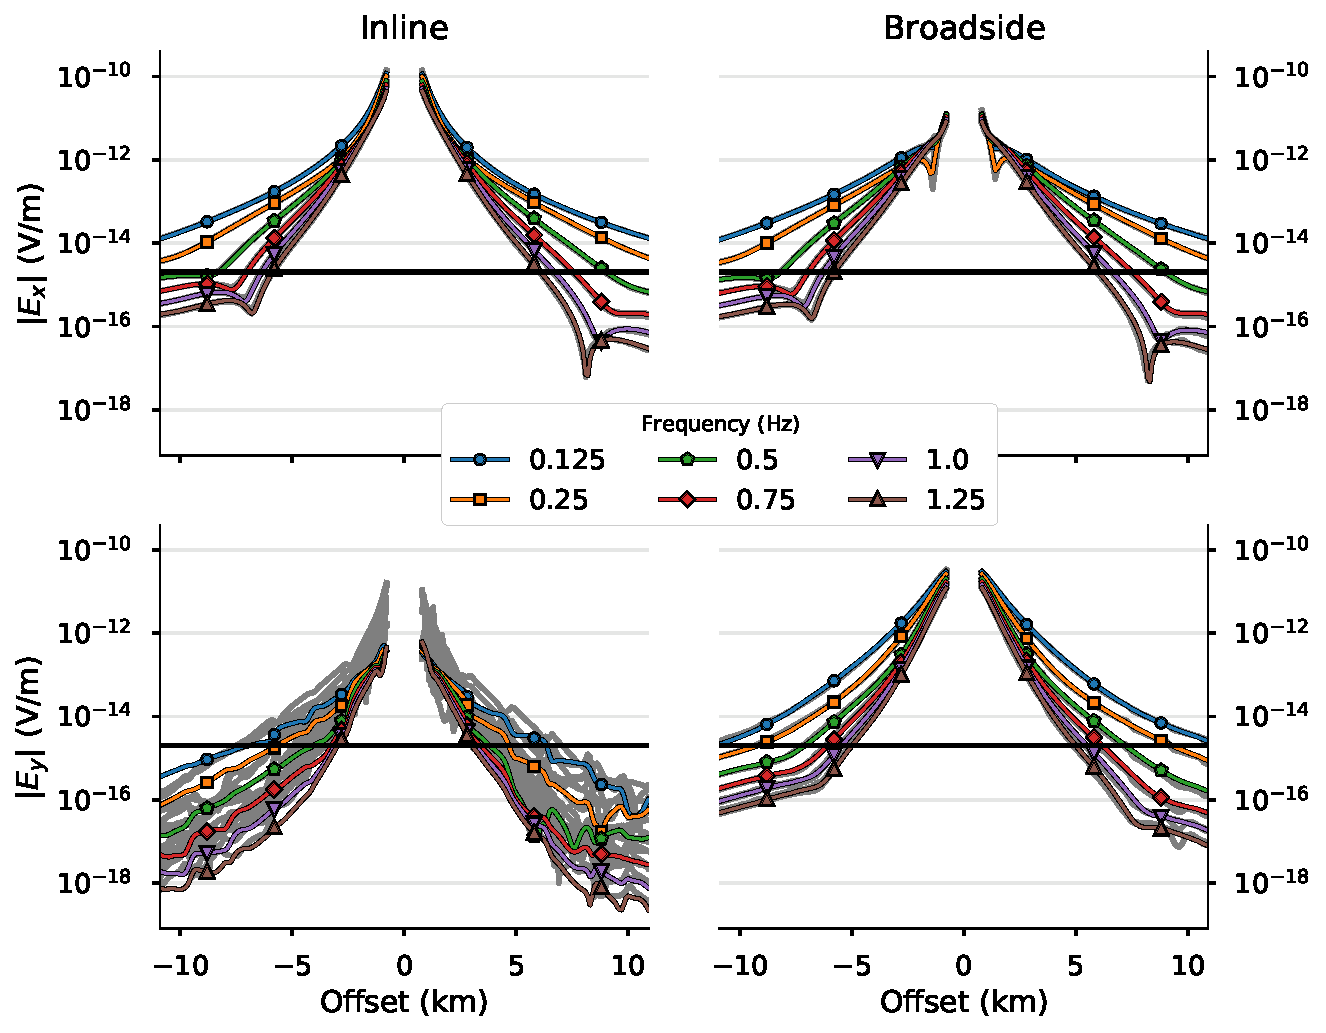
\includegraphics[width=\textwidth, trim=65 242 50 20, clip]{results-marlim-responses}\\[.5cm]
      %
      
\includegraphics[width=2.5cm]{Logo-PETGEM}
      %
  \end{columns}
  %
  \note{
    \begin{itemize}
      \item See you \alert{14th December}!
      \item Shown: Analytical verification; simple validation; complex
        validation
      \item Four codes, three different mesh types
      \item It is all about the discretization, the solvers themselves do
        basically the same
      \item Most time is spent in creating the appropriate discretization
      \item Performance depends mostly on the used solver
      \item Examples favoured rectilinear and octree meshes, as they were all
        regular cubes
      \item Examples favoured iterative solvers, as we only used one source;
        when computing many sources the direct solvers could re-use the
        factorisations
      \item We need more validations and benchmarks like this for CSEM
      \item More scenarios: air borne, strong topography, loops, conductor in
        a resistor, etc
      \item Reference model which is delivered on horizons and as functions
        instead of cubes
      \item More codes, other languages
    \end{itemize}
  }
\end{frame}

\end{document}
